\documentclass{article}


% if you need to pass options to natbib, use, e.g.:
%     \PassOptionsToPackage{numbers, compress}{natbib}
% before loading neurips_2022


% ready for submission
\usepackage{neurips_2022}
\usepackage{amsmath}


% to compile a preprint version, e.g., for submission to arXiv, add add the
% [preprint] option:
%     \usepackage[preprint]{neurips_2022}
% to compile a camera-ready version, add the [final] option, e.g.:
%     \usepackage[final]{neurips_2022}
% to avoid loading the natbib package, add option nonatbib:
%    \usepackage[nonatbib]{neurips_2022}


\usepackage[utf8]{inputenc} % allow utf-8 input
\usepackage[T1]{fontenc}    % use 8-bit T1 fonts
\usepackage{hyperref}       % hyperlinks
\usepackage{url}            % simple URL typesetting
\usepackage{booktabs}       % professional-quality tables
\usepackage{amsfonts}       % blackboard math symbols
\usepackage{nicefrac}       % compact symbols for 1/2, etc.
\usepackage{microtype}      % microtypography
\usepackage{xcolor}         % colors
\usepackage{graphicx}


\title{Optical Flow Regularization of Implicit Neural Representations for Video Frame Interpolation}

% The \author macro works with any number of authors. There are two commands
% used to separate the names and addresses of multiple authors: \And and \AND.
%
% Using \And between authors leaves it to LaTeX to determine where to break the
% lines. Using \AND forces a line break at that point. So, if LaTeX puts 3 of 4
% authors names on the first line, and the last on the second line, try using
% \AND instead of \And before the third author name.


\author{%
  David S.~Hippocampus\thanks{Use footnote for providing further information
    about author (webpage, alternative address)---\emph{not} for acknowledging
    funding agencies.} \\
  Department of Computer Science\\
  Cranberry-Lemon University\\
  Pittsburgh, PA 15213 \\
  \texttt{hippo@cs.cranberry-lemon.edu} \\
  % examples of more authors
  % \And
  % Coauthor \\
  % Affiliation \\
  % Address \\
  % \texttt{email} \\
  % \AND
  % Coauthor \\
  % Affiliation \\
  % Address \\
  % \texttt{email} \\
  % \And
  % Coauthor \\
  % Affiliation \\
  % Address \\
  % \texttt{email} \\
  % \And
  % Coauthor \\
  % Affiliation \\
  % Address \\
  % \texttt{email} \\
}


\begin{document}


\maketitle


\begin{abstract}
Recent works have shown the ability of neural implicit representations (NIR) to carry meaningful representations of signal derivatives.
In this work, we leverage this property to perform video frame interpolation
by explicitly constraining the derivatives of the NIR to satisfy the optical flow constraint equation.
We achieve state of the art video frame interpolation on limited motion ranges
using only a target video and its optical flow, without learning the interpolation operator from additional training data.
We further show that constraining the NIR derivatives not only
allows to interpolate intermediate frames but also improves the ability of narrow networks to fit observed frames,
which suggests potential applications to NIR optimization and video compression.
\end{abstract}

\section{Introduction}

% First paragraph general about the idea of using NIR to represent signals. [One paragraph, 4]
%% Many signal processing concepts defined in continuous spaces, but signal representation intrinsically discrete in digital computers
%% There is a problem with this:
%% In order to apply the infinitesimal quantities defined by theory to discrete sampled representations,
% unrealistic assumptions often have to be explicitly made, and rough heuristics employed.
%% The inability of rough heuristics to hold in generality have favored learning-based approaches

Many core concepts across the fields of signal processing are defined in terms of continuous functions and their derivatives:
surfaces are continuous manifolds in space,
motion is a rate of change in space through time, etc.
In contrast, the modern digital infrastructure is inherently discrete:
digital sensors capture discrete observations of the world sampled in time and space;
digital computers store and process discrete representations of signals.
In order to model continuous notions on discrete signal representations,
classical signal processing approaches have resorted to a variety of heuristics and assumptions,
often taking the form of constant first or second derivatives of the signal between consecutive observations.
The lack of generality of any such handcrafted heuristics,
combined with the ever improving quantitative results of Machine Learning (ML) approaches,
have led to the near ubiquitous use of ML approaches in recent signal processing research.
These approaches leverage large collections of data to infer statistical properties of signals instead of hand-crafted heuristics.
% With the advent of deep learning, recent state-of-the art approaches have moved away from explicitly applying theoretically derived heuristics,
% leveraging the flexibility of end-to-end representations, relying on large training datasets to decide on the heuristics.

% Then a historical approach to frame interpolation and Optical flow.
In computer vision, Video Frame Interpolation (VFI) is one task representative of such development.
VFI models aim to infer intermediate frames between consecutive frames of a video.
To do so, most successful approaches rely on the optical flow as an approximation of the motion field
to guide the interpolation of pixel intensities from the grid of two consecutive frames onto the pixel grid of intermediate frames.
Classical approaches formulate assumptions such as constant speed or acceleration of the motion field between consecutive frames [CITE].
The value of each pixel in the infered intermediate frame is computed by first shifting the pixel intesities of the observed frames following the
optical flow directions, and then interpolating the shifted pixel intensities onto the intermediate frame's pixel grid.
These approaches suffer from the following two limitations:

\begin{itemize}
\item Optical flow constraint used to infer the optical flow holds for limited situations. % Check me
\item Linear interpolation of pixel intesities along the optical flow directions does not hold in practice. % Check me
\end{itemize}

These limitations share a common root cause: discretization.
Indeed, both the optical flow constraint and the constant motion field assumption only truly hold at the infinitesimal scale,
for much smaller time deltas than typical FPS used in practice.

ML approaches [CITE] have instead proposed to learn the frame interpolation operator from large video collections,
without explicitly formulating any assumption on the optical flow.
While these approaches have achieved great success in terms of benchmark performance,
they are prone to generalization errors when applied to unseen videos. % Check me
Indeed differences between the training set distribution (i.e. VFI benchmark videos) and the target video distribution hinders the performance of ML approaches:
differences in the range of motion, exposure time and frame-per-second have been shown to limit the
generalization of state-of-the-art models to video frame interpolation in the wild [CITE]. %check me

% Implicit Neural Representation
%Meanwhile, another line of research has shown that deep architectures themselves provide powerful priors to represent signals (DIP, SIREN).
%Further efforts have been made to understand exactly what priors.
%In recent years, NNs have emerged as powerful parameterization of different signals.
%Why:
%- Depth provides more representational power.
%- Architecture provides inductive bias,
In the mean time, research on implicit representations seek better discrete representations of continuous signals.
In recent years Neural Implicit Representations (NIR), i.e. representing signals as Neural Networks (NN)
have been shown to offer several competitive advantages over explicit representations,
with notable early successes for 3D shape representations [CITE].
Of particular interest to us is the work of SIREN [CITE],
in which it has been shown that representing
signals using Multi Layer Perceptrons (MLP) with sine activation functions
carry meaningful representations of the signal derivatives.
Inspired by this work, we question wether such approach may be used to guide the interpolation
process of VFI by controlling the exact derivatives of the signal rather than finite differences,
thus avoiding the discretization pitfalls of traditional approaches.
We do so by constraining the derivatives of SIREN representations to satisfy the optical flow constraint,
i.e., to be orthogonal to the video's optical flow
(which we compute using existing state-of-the-art OF models).
We find that this approach outperforms most existing
machine learning-based approaches on small motion range benchmarks,
without relying on machine learning for the interpolation operator:
we simply regularize the implicit representation to satisfy the definition of the optical flow.
In this sense, our approaches is most similar to classical VIF approaches,
except that instead of wrapping the OF on discrete explicit frame representations,
we apply the optical flow constraint on the exact gradient of the the NIR.
Our method is thus not subject to any mismatch between training and test data.
Furthermore, our approach can sample any number of frame in-between the observed frames
due to the continuous nature of the representation.
In addition to its application to VFI, we also show that constraining the gradient
of the model also improves the ability of narrow MLPs to fit the signal,
suggesting potential applications in NIR optimization and video compression.

\begin{figure}[h]
\centering
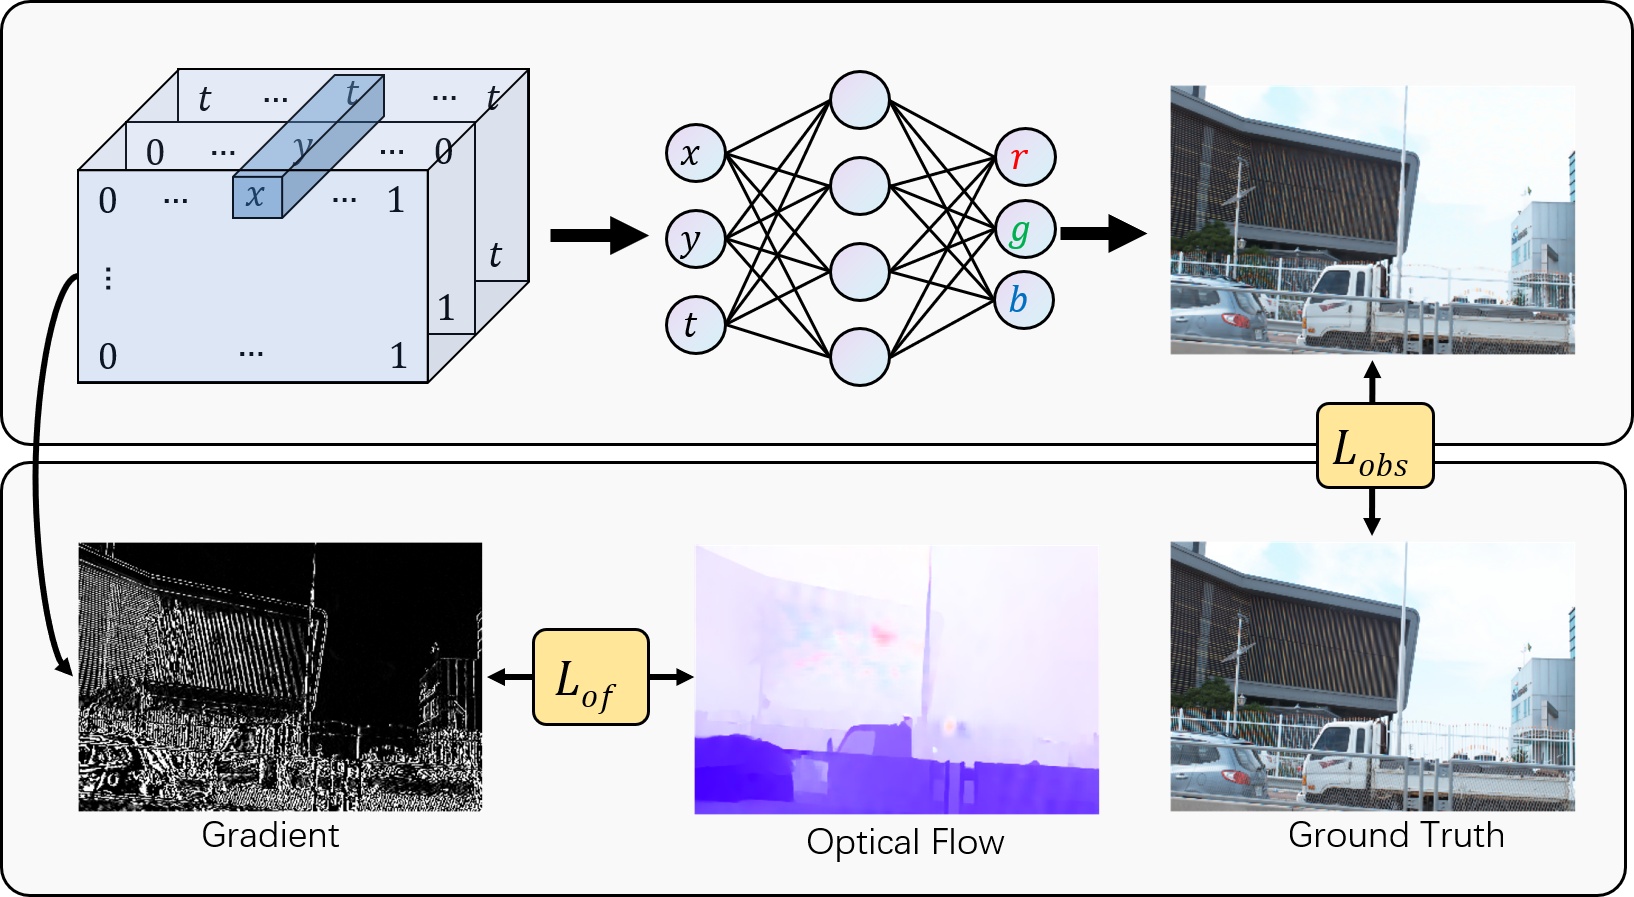
\includegraphics[width=0.8\textwidth]{Method}
\caption{Illustration of our approach}
\end{figure}

To summarize, the contributions of this work are:
\begin{itemize}
\item We propose a regularization method for SIREN which achieve state-of-the-art video frame interpolation on small motion ranges.
\item In contrast to other state-of-the art approaches, our approach does not rely on training on a large external training set.
It only relies on the target video and its estimated optical flow.
\item We show that our regularization approach not only helps generalizing to intermediate frame generalization
but also helps narrow models fit the observed frames.
\end{itemize}

On the other hand, our approach (in its current form) presents important limitations:

\begin{itemize}
\item It relies on an input optical flow, which is computed using existing ML-based model and thus suffers the limitations of ML approaches.
\item Optimization of the NIR is very time-consuming, which hinders our ability to work on full resolution videos for time constraints.
\item Our method currently only works on limited motion range. It does not match state-of-the art ML models on large motion ranges.
\end{itemize}

While we acknowledge the importance of the above limitations,
we believe these to not be fundamental limitations of our approach but rather important future NIR research directions.
We discuss these limitations at length and present possible axis to tackle them in Section XXX.
The remainder of this paper is organized as follows:
We briefly present some related work in Section XXX, the detail of our method in Section XXX,
and design several experiments to highlight the advantages of our approach in Section XXX.

\section{Related Work}

\textbf{Deep learning video interpolation.}
A number of deep learning models have been developed for video interpolation tasks.
Almost all models can be categorized as: optical flow based, and kernel based.

\textit{Optical Flow-Based.}
Optical flow-based approaches are the most popular in video frame interpolation.
The standard technique of video frame interpolation aims at explicitly estimating motion in the form of optical flow, warping two input frames to an intermediate frame, and synthesizing the occlusion region. The frames are constrained by the assumption of linear motion and constant luminance between them.
However, video interpolation of video frames is heavily dependent on the accuracy of optical flow.

The Super-SloMo \cite{jiang2018super} proposed by Jiang et,al. is a non-negligible work in the task of optical flow-based video frame interpolation.
Super-SloMo extends the U-Net architecture proposed by Liu et al \cite{liu2017video}.
The bilateral optical flow is calculated for the input two frames and approximates the key frame with the intermediate optical flow of the two frames.
Then the frames of the input are warped according to the obtained intermediate optical flow.

RRIN \cite{li2020video} mentioned that the estimation of intermediate frames in Super-SloMo works poorly near the boundaries because the optical flow is not locally smooth in these regions.
RRIN proposes to improve the accuracy of optical flow by residual learning.
BMBC \cite{park2020bmbc} adds two additional approximate vectors to Super-SloMo to make the bilateral motion estimation more accurate.


\textit{Kernel-Based.}
To avoid explicit motion estimation and warping stages, the kernel-based approach performs a convolution operation on the input frames and the output of the convolution is used as the result of interpolating the frames.
Niklaus et al. \cite{niklaus2017video1} proposed a fully convolutional deep neural network using a spatially adaptive convolutional kernel to perform the prediction of intermediate frames for two frames with consecutive inputs.
Niklaus et al. \cite{niklaus2017video2} improved their method by using a separable convolution with spatially adaptive one-dimensional convolutional kernel pairs estimated for each pixel, in reducing the parameters of the model.
The results of kernel-based methods for frame interpolation can be limited by the size of the kernel.

Lee et al. proposed Adacof \cite{lee2020adacof}, which can use any pixel at any position for convolution operation,
so that the convolution kernel is no longer limited to the local range.
And many methods residing in optical flow are defined as a special case of Adacof.
However, most kernel-based methods can only generate one intermediate frame, and if one wants to generate multiple intermediate frames, one needs to do it recursively.
EDSC \cite{cheng2021multiple} is the first kernel-based method proposed to generate multiple intermediate frames, but the results are not as good as the optical flow method.


\textbf{Implicit Neural Network Representation. (INR)}

INR use a neural network to represent an object approximately, which is essentially a way to parameterize the signal.
Since \cite{mildenhall2020nerf}, \cite{sitzmann2020implicit} was developed, INR has performed well in the areas of 3D vision tasks, images, and video.
The image and video tasks most relevant to this paper are around the direction of image/video compression.

COIN \cite{dupont2021coin} first proposed the use of INR to compress images, mapping pixel coordinates to RGB values.
COIN++ \cite{dupont2022coin++} cooperated with the meta-learning approach for image compression work based on COIN.
In the field of video compression, NeRV \cite{chen2021nerv} proposed by Chen et al. successfully encodes the video into a neural network, i.e., the content of the video is saved using a neural network.
Only the frame index of the model needs to be provided, and the corresponding RGB picture is output.
In other words, this makes it possible to output infinite frames of video using a neural network.
Although NeRV briefly attempts the task of performing video frame interpolation, this is not NeRV's main work.
The NRFF \cite{rho2022neural} proposed by Rho et al., which uses optical flow and residuals information for video compression, does not directly fit all frames.

Most related to our approach is the concurrent work by XX et al. \cite{shangguan2022learning}, which also uses INR for video interpolation tasks.
Their approach, CURE, uses machine learning.
It requires visual features of the video and does not fully map the pixel coordinates and frame positions of the video to RGB images.


\section{Method}

% We fit a video, and test on the middle frames
We consider a ground-truth video as a continuous signal $v$ mapping continuous spatial ($x$, $y$) and temporal ($t$) coordinates to RGB values:

\begin{equation}
\begin{aligned}
v:& \: (x, y, t) \rightarrow (R, G, B) \\
v:& \: \mathbb{R}^3 \rightarrow \mathbb{R}^3
\end{aligned}
\end{equation}

Our goal is to find a continuous function $f_{\theta}$, parameterized by a finite parameter set $\theta \in \Theta$,
with minimum distance $d$ to the ground-truth signal:

\begin{equation}
\begin{aligned}
f_{\theta}:& \:(x, y, t) \rightarrow (R, G, B) \\
s.t. \: \theta =& min_{\Theta} \iiint d(f_{\theta}(x,y,t), v(x,y,t)) dx dy dt
\end{aligned}
\end{equation}

where the distance function $d$ may either be the Peak Signal to Noise Ratio (PSNR) or the Structural Similarity Index Measure (SSIM).
To do so, we only have access to regularly sampled observation of the signal $v$
(i.e. the explicit representation of the video), which we denote as:

\begin{equation}
\begin{aligned}
&\mathcal{V} \in  \: \mathbb{R}^{T \times H \times W \times 3} \\
s.t. \: &\mathcal{V}_{xyt} =   v(x, y, t) %\: , \forall (x, y, t) \in \mathbb{N}^3
\end{aligned}
\end{equation}

% We start by showing that fitting a video does not naturally interpolate.
where $T$ represents the number of frames in the video, and $H \times W$ the spatial resolution.
We use SIREN as parameterized function class $f_{\theta}$.
The most straightforward way to approximate Equation 2 is to optimize the model parameters so as to fit the video frames,
using the following loss function we refer to as the observation loss:

\begin{equation}
\mathcal{L}_{obs} = \frac{1}{HWT} \sum_{x=1}^W\sum_{y=1}^H\sum_{t=1}^T || f_{\theta}(x,y,t) - \mathcal{V}_{xyt} ||^2
\end{equation}

\begin{figure}[t]
\centering
\includegraphics[width=0.8\textwidth]{"w_wo_OF"}
\caption{Illustration of NIR frame interpolation with and without optical flow regularization.
Without regularization (middle top), intermediate frames show unnatural high-frequency variations.
Regularizing the NIR to satisfy the optical flow constraint equation result in nicely interpolated frames (middle bottom).
}
\end{figure}

However, we found that optimizing the NIR to only minimize this observation loss leads to overfitting the observation with high temporal frequencies:
the intra-frame signal, which we aim to correctly recover, shows important deviations from the observed frames, as illustrated in Figure XXX.
This observation has lead us to consider fitting not only the signal itself, but to also constrain its derivatives.
In particular, we regularize the model so as to respect the optical flow constraint.

% But we show that regularizing with the OF does improve the interpolation
%$In computer vision, it is often used as as approximation of the motion field for 3d perception and navigation (cite),
%$or as a useful tool for video compression.
%The optical flow loss we use is defined as follows:

The optical flow constraint equation states that for an infinitesimal lapse of time $\delta t$,
the brightness of physical points perceived by a camera at arbitrary coordinates $(x,y,t)$ should remain constant.
In other words, given the displacement $(\delta x, \delta y)$ of a physical point in the image coordinate system,
the image brightness $v$ should remain constant:
\begin{equation}
v(x, y, t)=v(x + \delta x, y + \delta y, t + \delta t)
\end{equation}

Expressing movement as a ratio of displacement in time and abbreviating coordinates as $x=(x,y,t)$,
we can write the optical flow $F$ and the above constraint as:

\begin{equation}
\begin{aligned}
F(x)=(\frac{\delta x}{\delta t}, \frac{\delta y}{\delta t}, 1) \\
v(x)=v(x + F(x))
\end{aligned}
\end{equation}


We leverage this optical flow constraint equation to regularize the NIR.
Denoting the derivatives of the video signal as:

\begin{equation}
D(f, \theta, x, y, t)=\Big(\frac{\delta f_{\theta}(x,y,t)}{\delta x}, \frac{\delta f_{\theta}(x,y,t)}{\delta y}, \frac{\delta f_{\theta}(x,y,t)}{\delta t}\Big)
\end{equation}

And the optical flow as:


we can now define the optical flow regularization loss

\begin{equation}
\mathcal{L}_{of} = \frac{1}{HWT} \sum_{x \in W}\sum_{y \in H}\sum_{t \in T} | D(f, \theta, x, y, t) \cdot F(x, y, t) |
\end{equation}

This loss constrains the derivatives of the signal to be orthogonal to the optical flow and
can be intuitively understood as keeping constant brightness along the optical flow trajectories.
%thus dumping the high frequency temporal variations observed in Figure XXX.
The total loss we use to optimize the NIR is a weighted sum of these two terms:

\begin{equation}
\mathcal{L} = \lambda \mathcal{L}_{obs} + (1-\lambda) \mathcal{L}_{of}
\end{equation}

where $\lambda$ is a hyperparameter taking values between 0 and 1 whose impact we investigate in the following section.
The exactitude of the optical flow constraint at the infinitesimal scale plays in our favor:
As we regularize the true derivative of the signal representation,
we do not assume constant derivatives of the signal on any interval.
We believe this is the main factor behind our positive results.
On the other hand, the optical flow we used was estimated from discrete consecutive frames,
and thus does not represent the true infinitesimal motion field but an estimation of finite differences.
We discuss this limitation in Section XXX.

\section{Experiments}

Following previous works, we use the A, B and C dataset as benchmarks to compare to the state-of-the-art.
We run all additional experiments on the XXX video illustarted in Figure XXX.
Due to the time-consuming operation of optimizing SIREN representations, we optimize and evaluate all models on a XXX resolution.
For the A dataset, we follow the standard 8 video split XXX.

Unless specified other-wise, all experiments are run with a SIREN of depth XXX and width XXX.
We use an omega of XXX and a lambda of XXX.
We optimize the models using the Adam optimizer using a cosine learning rate with maximum learning rate of XXX during XXX epochs.

We start by showing the impact of controling the fit to high frequency without the optical flow loss in section XXX.
We show that while limiting the frequency fitted does improve generlization, it does not allow to reach
the same accuracy as optical flow regularization, showing that OF regularization does more than just limiting the fitted frequencies.

In Section XXX, we compare our results to state of the art quantitatively on standard benchmarks.
We show that our approach achieves state-of-the-art resuklts on low-range motion datasets, but underperforms existing methods on the high-range motion dataset.
We present an ablation in Section XXX, providing inisight and appropriate settings on the different model hyperparameters and a qualitative analysis of our results in Section XXX.

Finally, we report a surprising additional result in Section XXX:
We show that XXX.

\subsection{Optical Flow constaint and High Frequencies}

Figure 2 illustrates the fact that applying the optical flow constraint smoothes out the high-frequency variations
from the intermediate frames of vanilla SIREN representations.
We start by questioning wether the OF constraint does more than simply removing the high frequency variations of the representation.
To do so, we compare the results of vanilla SIREN representations geared towards different frequency and compare the
best obtained results to OF-constrained representations.
We constrain the SIREN frequency by varying their $\omega$ parameter,
and report our comparison in Figure XXX.

\begin{figure}[t]
\centering
\includegraphics[width=0.5\textwidth]{"omega_wo_of"}
\caption{NEED TO SHOW TRAINING CURVE AND THRESHOLD ATTAINED BY OF}
\end{figure}

While constraining the high frequency with low $\omega$ does improve the ability to interpolate intermediate frames,
vanilla SIREN models remain well under the OF-constrained representations,
confirming than the OF constraint provides more simply restricting the high temporal frequencies.

\subsection{State of the art models}

Table XXX quantitatively compare the results of our model to state-of the art VFI models on different datasets.
We show that


\begin{table}[]
\centering
\caption{Quantitative comparison to state-of-the-art VFI on limited motion range benchmarks. Results are formatted as PSNR / SSMI.}
\begin{tabular}{l | l | l }
 &  Adobe-240FPS  [XXX] &  X4K [XXX]  \\
\hline
Super-SloMo [XXX] &  27.77/0.8866 & 27.38/0.8527  \\
RRIN [XXX]  & 32.37 / 0.9624 & 30.70 / 0.9270  \\
BMBC [XXX]  & 27.83 / 0.9172 & 27.42 / 0.8585   \\
AdaCof [XXX] & 35.50 / 0.9684 & 34.61 / 0.9218 \\
ABME   [XXX] & 35.28 / 0.9669 & 34.30 / 0.9195 \\
FILM   [XXX] &	35.97 / 0.9710 & \textbf{35.14} / 0.9397 \\
Ours	& \textbf{36.52} / \textbf{0.9770} & 35.06/ \textbf{0.9441} \\
\end{tabular}
\end{table}



\begin{table}[]
\centering
\caption{Quantitative comparison to state-of-the-art VFI on large motion range benchmarks. Results are formatted as PSNR / SSMI.}
\begin{tabular}{l | l }
	    &   ND Scene [XXX] \\
\hline
V-NF        &  23.30 / 0.7260 \\
NSFF [10]   & 28.03 / 0.9250 \\
CURE [11]   & \textbf{36.91} / \textbf{0.9843} \\
Ours	      & 29.22 / 0.9215
\end{tabular}

\end{table}



\subsection{Ablation study}

Next, we highlight the



\subsection{Qualitative Analysis}

%
Ask Sho-kun.

\subsection{Video fitting}



\section{Limitations}

While we believe our results to be very encouraging, the proposed approach is not yet practical.
Here, we discuss what we believe to be the three main limitations of, and possible solutions to, our approach

\textbf{Slow optimization process.} Fitting XXX frames of a video at XXX resolution currently takes XXX hours on a XXX GPU using Pytorch.
This computation time is a huge draw back as it limits our ability to process full resolution video as well as
to explore different hyper parameters and variants of the methods.
We expect new methods speeding up the convergence of video NIR to be very benefic to this line of research.
Given recent successes of NIR approaches to high impact applications (i.e., video compression [CITE]),
We hopefully expect to see advances in NIR optimisation research.

% Relying on optical flow model.
\textbf{Reliance on trained optical flow model.}
SIREN models allow us to apply the optical flow on the exact derivaties of the signal,
thus bypassing the heuristics of classical approach without relying on machine learning.
The optical flow we use, however, is given by a trained ML model, which raises two problems:
it is subject to generalization error, and the flow is computed on discrete samples and then subject to
undesirable changes in illumination and occlusion.
Future work will aim to bypass our reliance on ML-based OF using proxy constraints on the exact derivatives.

\textbf{Inability to interpolate high motion range videos.}
In its current form, our approach only regularizes observed frames of the video.
This has proven sufficient to reach state-of-the art on low motion ranges but is not sufficient for large motions.
% However, there is still a lot of room for improvement,
For larger motions several improvements can be considered, most notably by regularizing intermediate frames.
Texture conservation in intermediate frames, interpolated optical flows.

\section{Conclusion}

In this paper, we have shown that regularizing NIR using the optical flow constraint equation
enabled VFI without relying on ML to perform the interpolation step.
We show that this approach is sufficient to reach state-of-the-art interpolation
on low montion ranges

\section*{References}

\medskip

{
\small


[1] Alexander, J.A.\ \& Mozer, M.C.\ (1995) Template-based algorithms for
connectionist rule extraction. In G.\ Tesauro, D.S.\ Touretzky and T.K.\ Leen
(eds.), {\it Advances in Neural Information Processing Systems 7},
pp.\ 609--616. Cambridge, MA: MIT Press.


[2] Bower, J.M.\ \& Beeman, D.\ (1995) {\it The Book of GENESIS: Exploring
  Realistic Neural Models with the GEneral NEural SImulation System.}  New York:
TELOS/Springer--Verlag.


[3] Hasselmo, M.E., Schnell, E.\ \& Barkai, E.\ (1995) Dynamics of learning and
recall at excitatory recurrent synapses and cholinergic modulation in rat
hippocampal region CA3. {\it Journal of Neuroscience} {\bf 15}(7):5249-5262.
}


\end{document}
